\section{Navigation}

As our website will be used by cell phones or computers, it is important to develop a design which supports user navigation, printing, etc. For this, we will use a single-screen design and navigation tools.

\subsection{General design}

Nowadays, there are a lot of devices which are able to access websites and each of them has a different screen size. It is better to use a single-screen design than a predefined size of screens (for example 800x600). It assures that the navigation is usable on various devices. 

It is also important to establish a compromise between separate pages and scrolling on a long page. Since users don't like to scroll pages, but if there are too many pages, he will be lost in the number of different pages.


\subsection{Global systems}

We placed our logo at the top on the left side. This will be included on every subpage to ensure that the user always knows on which website he is.
Also at the top of every page and directly to the right of the website logo, is the global navigation menu. As defined in section \textit{5.3.1}, the menu (figure \ref{fig:globalMenu}) is composed of the followings groups: Boy, Girl, Clearance and Second Hand.

\begin{figure}[h!]
  \centering  
  
\includegraphics[width=0.5\textwidth]{Images/globalMenu.jpg}                
  \caption{Global navigation menu}
  \label{fig:globalMenu}
\end{figure}


\subsection{Local systems}
The local menu appears, as a cascading menu, when the user moves the mouse on one of the global menu items. It is also on the left of every page (except the home page) below the logo and the global menu. As soon as the user selects one of the entries, he has access to the subgroups of this category, as defined in section \textit{5.3.1}. For each subgroup (except Dresses, Bodysuits and Pajamas), you can also select a subsubgroup in the cascading menu. The figure \ref{fig:localMenu} shows examples for the Boy's local menu on the left.

\begin{figure}[ht!]
  \centering
  \subfloat[Sublocal menu for Tops]{\label{fig:localMenuTops}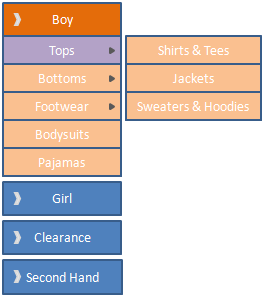
\includegraphics[width=0.35\textwidth]{Images/localMenuTops.png}}                
  \subfloat[Sublocal menu for Bottoms]
  {\label{fig:localMenuBottoms}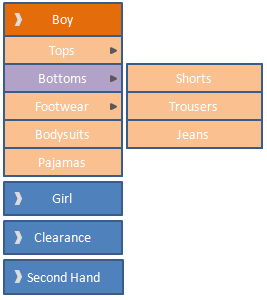
\includegraphics[width=0.35\textwidth]{Images/localMenuBottoms.png}}
  \subfloat[Sublocal menu for Footwear]{\label{fig:localMenuFootwear}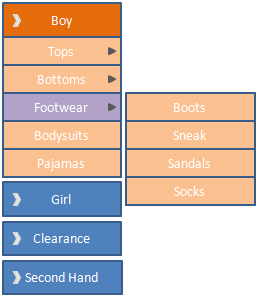
\includegraphics[width=0.35\textwidth]{Images/localMenuFootwear.png}}
  \caption{Local menu for Boys}
  \label{fig:localMenu}
\end{figure}

\subsection{Contextual and Supplemental systems}
Contextual navigation systems like hypertext links or associative links, appear within the textual description to a selected item. Additionally, there are "also bought" and "you may also like" lists, with which users can see what other people bought with the selected product, or what the underlying database recommends. Users can also use supplemental navigation tools like the "Search bar" and "Breadcrumbs", which are very useful for finding where they are and offer quick access to specific items.


